% Chapter Template

\chapter{Method} % Main chapter title

\label{ChapterX} % Change X to a consecutive number; for referencing this chapter elsewhere, use \ref{ChapterX}

%----------------------------------------------------------------------------------------
%	SECTION 1
%----------------------------------------------------------------------------------------

\section{Disentangled Semantic Topic Model}

We construct the Disentangled Semantic Topic Model (DSTopic) as a method to extract multi-faceted knowledge from complex and informative textual data. The DSTopic model is specifically designed to address the limitations of traditional topic models, which often rely on the assumption that there is only a single generative process underlying the data. In contrast, DSTopic proposes a disentangled multi-view generative framework, allowing the model to capture and represent different semantic aspects or facets of documents simultaneously. By doing so, DSTopic is able to provide a more comprehensive and structured understanding of the information contained within a collection of texts. However, optimizing the likelihood function in DSTopic directly is generally intractable due to the complexity of the model and the high-dimensional nature of textual data. To address this challenge, we adopt variational inference, which offers an efficient and scalable way to approximate the posterior distributions required for model estimation. In our implementation, DSTopic utilizes a Disentangled Semantic Variational Autoencoder (DSVAE) as its core component, which helps to separate the semantic representations of the data into distinct, meaningful components. In addition, we incorporate a vocabulary clustering module, which further enhances the semantic disentanglement by grouping similar words together. This combined approach enables DSTopic to achieve more accurate and interpretable topic representations, making it a powerful tool for analyzing and understanding large-scale text corpora.


%-----------------------------------
%	SUBSECTION 1
%-----------------------------------
\subsection{Disentangled Generative Process}
\label{chapter:generation}

Unlike traditional topic models that generate documents from a single topic model, DSTopic assumes that each document is generated by topic model with $ H $ distinct views. Each of the $ H $ views is associated with a distinct subset of the vocabulary $\mathcal{V}^{(h)}$. These subsets are disjoint (i.e., they do not share words), ensuring that each view captures an independent semantic aspect of the document. The full vocabulary is reconstructed as the union of all subsets: $ \bigcup_{h=1}^H \mathcal{V}^{(h)} = \mathcal{V} $. 
Accordingly, the $ h $-th view maintains independent topic embeddings $ \alpha^{(h)} \in \mathbb{R}^{\frac{K}{H} \times D_{TM}} $ and word embeddings $ \rho^{(h)} \in \mathbb{R}^{V^{(h)} \times D_{TM}} $, where $ V^{(h)} $ is the size of the corresponding vocabulary set $ \mathcal{V}^{(h)} $. The topic-word distributions of the $ h $-th view, denoted as $ \beta^{(h)} \in \mathbb{R}^{\frac{K}{H} \times V^{(h)}} $, can be computed as: $ \beta^{(h)} = \text{Softmax}(\alpha^{(h)} \rho^{(h)\mathrm{T}}) $. 
Given this framework, the disentangled generative process for document $ t_j $ is as follows:
\begin{enumerate}
    \item For each view $h = 1, \dots, H$:
    \begin{enumerate}
        \item Draw view-aware topic proportions $ \theta_{j}^{(h)} \sim \mathcal{LN}(\mathbf{0}, \mathbf{I}) $ .
    \end{enumerate}
    
    \item For each word $ b_{j,v} $ in the document $ t_j $:
    \begin{enumerate}
        \item Determine the view $ h_{j,v} $ to which the word $ \mathbf{b}_{j,v} $ belongs.
        \item Draw a topic assignment $ \mathbf{z}_{j,v} \sim \text{Cat}(\theta_{j}^{(h_{j,v})}) $.
        \item Draw the word $ b_{j,v} \sim \text{Cat}(\beta_{\mathbf{z}_{j,v}}^{(h_{j,v})}) $.
    \end{enumerate}
\end{enumerate}

In step (1), DSTopic derives the view-aware topic proportions $ \theta_{j}^{(h)} $ for $ h \in [1, 2, \cdots, H] $ from the logistic-normal distribution for the subsequent generation. In step (2), DSTopic first determines the view $ h_{j,v} $ associated with the word $ b_{j,v} $, representing documents as distributions over the topics in $ h_{j,v} $ and drawing a topic assignment for each observed word.


%-----------------------------------
%	SUBSECTION 2
%-----------------------------------

\subsection{Inference and Estimation of the Disentangled Generative Process}
Following the introduction of the disentangled generative process, DSTopic derives the likelihood of optimizing the parameters involved. Specifically, we aim to maximize the marginal likelihood of the documents, formulated as follows:
\begin{align}
    \mathcal{L}(\bm{\alpha}, \bm{\rho}) = \sum_{j=1}^J \sum_{h=1}^H \log p(\mathbf{b}_j^{(h)} | \alpha^{(h)}, \rho^{(h)}),
    \label{eq:likelihood}
\end{align}
where $ \bm{\alpha} = \{\alpha^{(1)}, \alpha^{(2)}, \cdots, \alpha^{(H)}\} $ denotes the set of topic embeddings for all views of the topic model, $ \bm{\rho} = \{\rho^{(1)}, \rho^{(2)}, \cdots, \rho^{(H)}\} $ denotes the vocabulary embedding set for all views, and $ \mathbf{b}_j^{(h)} \in \mathbb{R}^{V^{(h)}} $ represents the Bag-of-Words (BoW) vector under the view $ h $. We introduce a challenging integral over the view-aware topic proportions $ \theta^{(h)} $ and rewrite the probability term as:
\begin{align}
\small
    p(\mathbf{b}_j^{(h)} | \alpha^{(h)} \rho^{(h)}) = \int p(\theta_j^{(h)}) p(\mathbf{b}_j^{(h)} | \theta_j^{(h)}, \alpha^{(h)}, \rho^{(h)}) \, \text{d}\theta_j^{(h)},
\end{align}
The conditional distribution of the BoW vector can be expressed as:
\begin{align}
\small 
    p(\mathbf{b}_j^{(h)} | \theta_j^{(h)}, \alpha^{(h)}, \rho^{(h)}) = \theta_j^{(h)} \beta_j^{(h)} = \theta_j^{(h)} \text{Softmax}(\alpha^{(h)} \rho^{(h)\mathrm{T}}),
\end{align}

However, due to the unknown distribution $ p(\theta_j^{(h)}) $ and the intractable integral, the likelihood in Eq.~\ref{eq:likelihood} remains intractable. To address this issue, ETM \cite{dieng2020topic} introduces a variational distribution $ q(\theta_j; \mathbf{b}_j, \nu) $, where $ \nu $ represents the parameters of the inference network used to derive $ q(\theta_j) $ (noting that there is no disentangled modeling in ETM, so we omit the superscript). However, this variational distribution leverages the BoW vector, neglecting the semantic information present in the document. To address this limitation, we introduce a new variational distribution $ q(\theta_j^{(h)}; \mathbf{t}_j, \nu^{(h)}) $ for a better understanding of the semantic information in the documents. Specifically, $ q(\theta_j^{(h)}; \mathbf{t}_j, \nu^{(h)}) $ is a Gaussian distribution, with its mean and variance derived from an inference network with parameters $ \nu^{(h)} $. This inference network takes the semantic embedding $ \mathbf{t}_j $ of document $ t_j $ as input and outputs the mean and variance of $ \theta_j^{(h)} $.


After introducing this variational distribution, we derive the Evidence Lower Bound (ELBO) to approximate the original likelihood for optimizing both the topic parameters and the variational parameters. The ELBO is formulated as:
\begin{align}
    \mathcal{L}(\bm{\alpha}, \bm{\rho}, \nu) = \sum_{j=1}^J \sum_{h=1}^H &\mathbb{E}_{q(\theta_j^{(h)}; \mathbf{t}_j, \nu^{(h)})} p(\mathbf{b}_j^{(h)} | \theta_j^{(h)}, \alpha^{(h)} \rho^{(h)})  \notag \\
    &- \text{KL}(q(\theta_j^{(h)}; \mathbf{t}_j, \nu^{(h)}) || p(\theta_j^{(h)})),
    \label{eq:elbo}
\end{align}
where $ p(\theta_j^{(h)}) $ is a prior distribution defined as a standard Gaussian distribution $ \mathcal{N}(\mathbf{0}, \mathbf{I}) $, and $\text{KL}(\cdot ||\cdot)$ denotes the KL-divergence.

%-----------------------------------
%	SUBSECTION 3
%-----------------------------------

\subsection{Implementation of Disentangled Generative Process}
In this section, we provide a detailed implementation of the Disentangled Semantic Topic Model (DSTopic), as illustrated in Figure~\ref{fig:architecture}. The implementation consists of two core modules: Vocabulary Clustering and Disentangled Semantic VAE (DSVAE).

\noindent \textbf{(1) Vocabulary Clustering} aims to partition the original vocabulary set into multiple sub-vocabulary sets. We introduce $H$ view embeddings, denoted by $\gamma \in \mathbb{R}^{H \times D_{TM}}$, and compute matching scores between views and words using cosine similarity  $\mathbf{S}' = \rho / |\rho| \left(\gamma /|\gamma|\right)^{\mathrm{T}}$,
%$\mathbf{S}' = \frac{\rho}{|\rho|} \left(\frac{\gamma}{|\gamma|}\right)^{\mathrm{T}}$,
where $\mathbf{S}' \in \mathbb{R}^{V \times H}$ denotes the similarity matrix between views and words, $\gamma$ and $\rho$ denote the embeddings of views and words, respectively, and $|\cdot|$ denotes the L-2 norm of the raw vector of the matrix. To obtain hard cluster labels, we apply the Gumbel-Softmax activation function \cite{jang2016categorical}, formulated as:
\begin{align}
\small
    \mathbf{S} = \frac{\exp(\log \mathbf{S}' - \log(-\log \mathbf{U}))}{\sum_{h=1}^H \exp(\log \mathbf{S}_{\cdot,h}' - \log(-\log \mathbf{U}_{\cdot,h}))} ,
    \label{eq:gumbel}
\end{align}
where $\mathbf{U} \in \mathbb{R}^{V \times H}$ denotes a random matrix sampled from the $\text{Gumbel}(0,1)$ distribution with the same dimensions as the score matrix $\mathbf{S}$, and $\mathbf{S}_{\cdot,h}$ and $\mathbf{U}_{\cdot,h}$ denote the column vectors of matrices $\mathbf{S}$ and $\mathbf{U}$, respectively. After applying Eq.~\ref{eq:gumbel}, each row of $\mathbf{S}$ is a one-hot vector indicating the view to which each word belongs.

\textit{Preventing View Collapse:} During the training of the vocabulary clustering module, we observed the view collapse issue, where a single view contains most words in the vocabulary while other views contain very few words. This collapse hinders further knowledge disentanglement learning. To mitigate this issue, we introduce a variance normalization term, which calculates the variance of the number of words across different views. Specifically, the normalization term $\mathcal{L}_{var}$ is defined as:
\begin{align}
\small
    \mathcal{L}_{var} = \left(\sum_{v=1}^V \mathbf{S}_{v, \cdot} - \frac{\sum_{h=1}^H \sum_{v=1}^V \mathbf{S}_{v, h}}{H}\right)^2 ,
\end{align}
where $\mathbf{S}_{v, \cdot}$ represents the raw vector of matrix $\mathbf{S}$. The first term represents the total number of words belonging to all views, while the second term calculates the mean size of the views.

\noindent \textbf{(2) Disentangled Semantic VAE (DSVAE)} implements the DSTopic using a VAE-based framework, which consists of an Inference Layer (Encoder), a Latent Sampling Layer, and a Generation Layer (Decoder). Specifically, for document $t_j$, as shown in Figure~\ref{fig:architecture}, the \textit{inference layer} aims to extract the view-aware topic embedding $\mathbf{z}_j^{(h)}$ from the semantic embedding $\mathbf{t}_j$, denoted by $\mathbf{z}_j^{(h)} = f_{in}^{(h)}(\mathbf{t}_j)$, where $f_{in}^{(h)}$ is the inference network for view $h$. 

Next, the \textit{latent sampling layer} learns the mean and variance of the view-aware topic proportion $\theta'^{(h)}_j$, denoted by $\theta'^{(h)}_j \sim \mathcal{N}(f_{mean}^{(h)}(\mathbf{z}_j^{(h)}), f_{var}^{(h)}(\mathbf{z}_j^{(h)}))$. To preserve the gradient, we adopt the reparameterization trick following conventional VAE \cite{kingma2013auto} to obtain the sampled $\theta'^{(h)}_j$. A softmax normalization is then applied on $\theta'^{(h)}_j$ to obtain $\theta^{(h)}_j$, ensuring that the probabilities sums to 1. 

Finally, the \textit{generation layer} follows the disentangled generative process presented in Section~\ref{chapter:generation} to reconstruct the view-aware BoW vector $\hat{\mathbf{b}}_j^{(h)}$.

\begin{figure}[t]
    \centering
    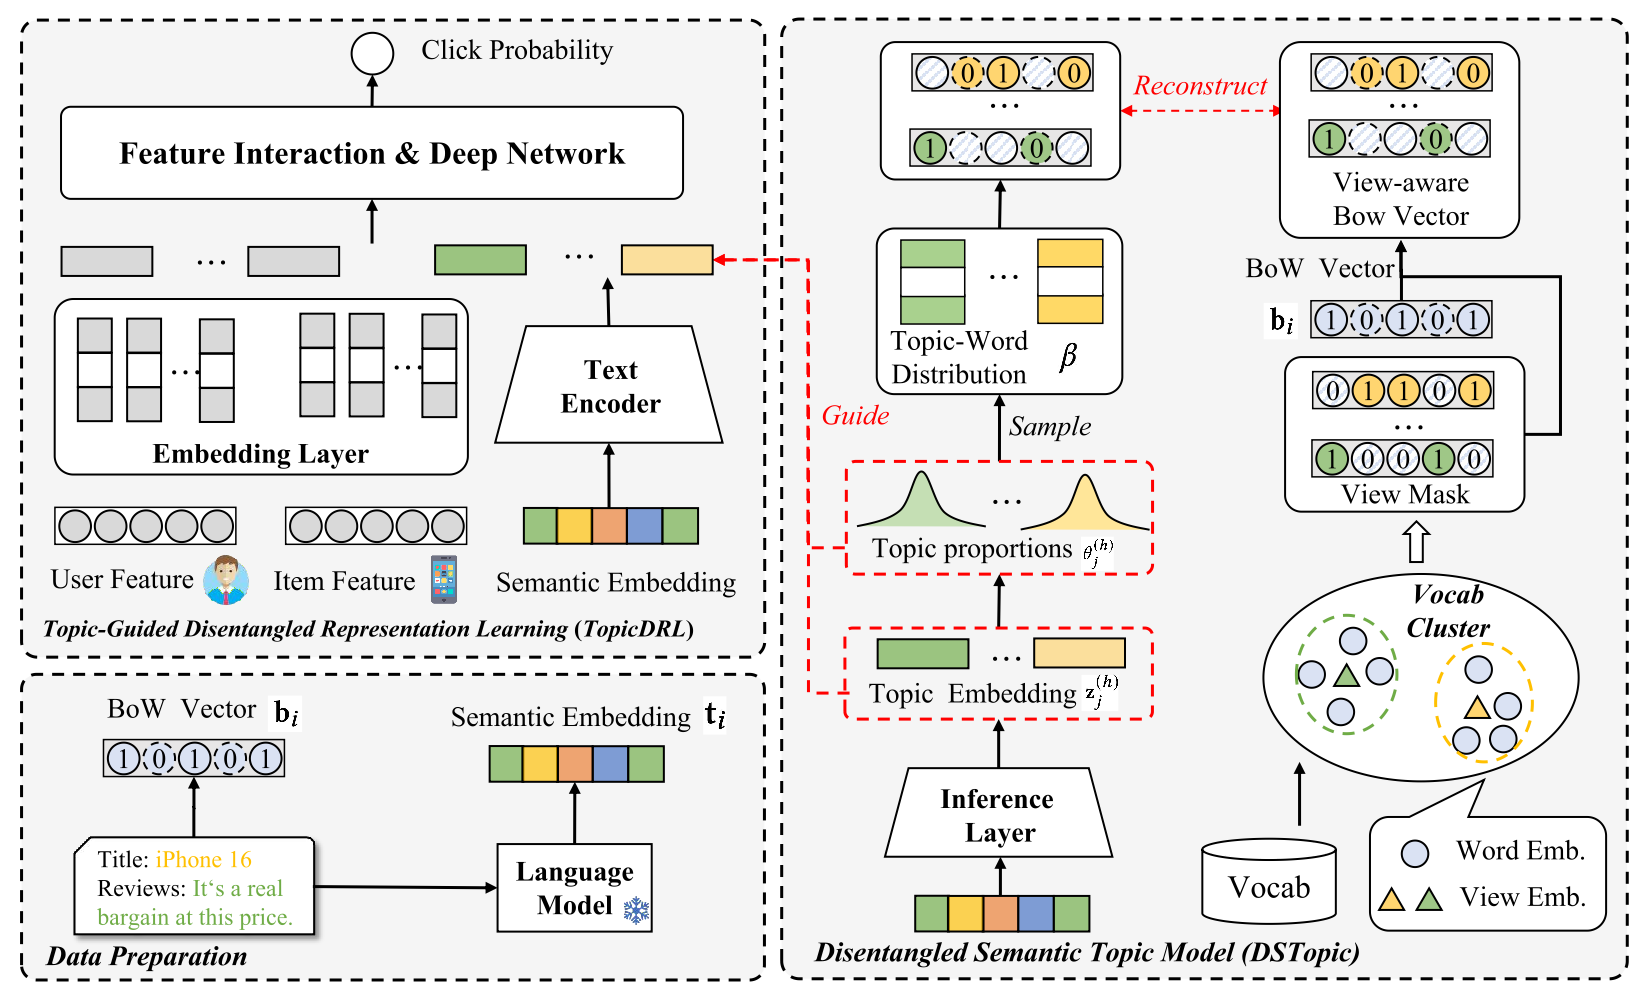
\includegraphics[width=0.9\linewidth]{Figures/Chapter3/fig2.png}
    \caption{Overall architecture of MSD-CTR, which consists of two key components: (1) DSTopic, responsible for extracting disentangled topic representations, and (2) TopicDRL, which integrates these representations into CTR prediction.}
    \label{fig:architecture}
\end{figure}

%----------------------------------------------------------------------------------------
%	SECTION 2
%----------------------------------------------------------------------------------------

\section{Topic Guided Disentangled Representation Learning}

To incorporate multi-faceted knowledge from our disentangled topic model into the CTR prediction task, we initially attempted a straightforward approach by directly integrating the learned view-aware topic embeddings $\mathbf{z}^{(h)}$ into the existing feature set used for prediction. The intuition behind this direct integration was that the topic embeddings, which capture semantic aspects of documents, would naturally enhance the model's ability to predict click-through rates by providing additional contextual information. However, despite this reasonable assumption, this naive operation did not yield the significant performance improvements we expected. In fact, in some experimental settings, directly incorporating these topic embeddings actually introduced negative effects, leading to decreased prediction accuracy compared to baseline models without topic information.

This counterintuitive phenomenon can be attributed to several underlying factors. First and most importantly, the information that is relevant and useful for document generation within the topic model framework is not entirely aligned with the information that is optimal for CTR prediction tasks. While topic models are designed to capture the semantic structure and thematic content of documents, CTR prediction requires understanding user behavior patterns, engagement signals, and factors that influence clicking decisions. These two objectives, though related, operate on different levels of abstraction and require different types of information. Second, directly feeding the topic embeddings $\mathbf{z}^{(h)}$ into the CTR prediction model may inadvertently overlook beneficial information that could be extracted from the topic representations through more sophisticated processing. At the same time, this direct approach may introduce unnecessary noise and irrelevant details that are useful for topic modeling but detrimental to CTR prediction performance.

Given these challenges and the suboptimal results from the direct integration approach, we recognized the need for a more sophisticated method to bridge the gap between topic modeling and CTR prediction. Therefore, we propose the Topic Guided Disentangled Representation Learning (TopicDRL) framework as a refined and more principled alternative to directly using the raw topic embeddings $\mathbf{z}^{(h)}$. The TopicDRL framework is specifically designed to selectively extract and transform the relevant information from the topic embeddings while filtering out noise and irrelevant details. This approach allows us to leverage the multi-faceted knowledge captured by our disentangled topic model in a way that is more aligned with the requirements and objectives of CTR prediction tasks.

TopicDRL encourages disentangled embeddings learning from the semantic embedding $\mathbf{t}_i$, denoted as:
$[\tilde{\mathbf{t}}_i^{(1)}, \tilde{\mathbf{t}}_i^{(2)}, \cdots, \tilde{\mathbf{t}}_i^{(H)}] = f_{text}(\mathbf{t}_i)$
where $\tilde{\mathbf{t}}_i^{(h)} \in \mathbb{R}^D$ represents the disentangled embedding, which has the same dimension as other features in conventional CTR prediction, and $H$ is the number of views, consistent with the number of views in DSTopic. The estimated CTR is computed as:
$
\hat{y}_i = f_{CTR}(\tilde{\mathbf{t}}_i^{(1)}, \tilde{\mathbf{t}}_i^{(2)}, \cdots, \tilde{\mathbf{t}}_i^{(H)}, \mathbf{e}_{i,1}, \mathbf{e}_{i,2}, \cdots, \mathbf{e}_{i,m}).
$



To effectively guide the learning of disentangled embeddings, we introduce two types of alignment losses: an individual-level alignment loss and an intra-view contrastive loss. The \textbf{individual-level alignment loss} $\mathcal{L}_{ind}$ uses the learned multi-view topic embeddings $\mathbf{z}_i^{(h)}$ to supervise the learning of the semantic embeddings $\tilde{\mathbf{t}}_i^{(h)}$. Specifically, $\mathcal{L}_{ind}$ is defined as:
\begin{align}
    \mathcal{L}_{ind} = \sum_{i=1}^N \sum_{h=1}^H |\tilde{\mathbf{t}}_i^{(h)} - f_{tma}(\mathbf{z}_i^{(h)})| ,
\end{align}
where $f_{tma}$ is an adapter implemented by a fully connected network to align the embedding dimensions, $|\cdot|$ is the L-2 norm, and $N$ is the size of the dataset. This loss encourages the semantic embeddings $\tilde{\mathbf{t}}_i^{(h)}$ to focus on shared facet information. Since the disentangled topic embeddings capture different views of knowledge from the textual information, $\mathcal{L}_{ind}$ helps the semantic embeddings $\tilde{\mathbf{t}}_i^{(h)}$ learn in a disentangled embedding space.


Additionally, to normalize the disentangled semantic embeddings learning $\tilde{\mathbf{t}}_i^{(h)}$, TopicDRL introduces an \textbf{intra-view contrastive loss}. This loss assumes that if two items have similar topic distributions in a specific view, their corresponding semantic embeddings should also be similar. Specifically, the intra-view contrastive loss $\mathcal{L}_{int}$ is defined as:
\begin{align}
\small
    \mathcal{L}_{int} = \sum_{h=1}^H \sum_{i=1}^N \frac{\sum_{i'=1}^N a_{i,i'} \exp(\text{sim}(\tilde{\mathbf{t}}_i^{(h)}, \tilde{\mathbf{t}}_{i'}^{(h)}))}{\sum_{i'=1}^N \exp(\text{sim}(\tilde{\mathbf{t}}_i^{(h)}, \tilde{\mathbf{t}}_{i'}^{(h)}))} ,
\end{align}
where $\text{sim}(\cdot, \cdot)$ is a similarity function implemented using cosine similarity, and $a_{i,i'}$ is a weight that estimates the relationship between the textual items $t_i$ and $t_{i'}$, calculated based on the similarity of their topic distributions:
\begin{align}
\small
    a_{i,i'} = \frac{\text{sim}(\mathbf{z}_i^{(h)}, \mathbf{z}_{i'}^{(h)})}{\sum_{i'=1}^N \text{sim}(\mathbf{z}_i^{(h)}, \mathbf{z}_{i'}^{(h)})} ,
\end{align}
Due to the large dataset size $N$, $\mathcal{L}_{int}$ is implemented at the batch level. This loss encourages intra-view relations by pulling semantic embeddings with similar topic distributions closer together while pushing those with dissimilar topic distributions apart.

In addition to the alignment losses, the main CTR prediction loss is defined as a binary cross-entropy loss $\mathcal{L}_{BCE} = - \sum_{i=1}^N [y_i \log \hat{y}_i + (1-y_i)\log (1-\hat{y}_i)]$.
The overall CTR prediction network is trained under the combined CTR loss:
$
\mathcal{L}_{CTR} = \mathcal{L}_{BCE} + \mathcal{L}_{ind} + \mathcal{L}_{int}.
$